\documentclass[10pt,a4paper,oneside]{article}
\usepackage[utf8]{inputenc}
\usepackage{draftwatermark} % 设置水印
\SetWatermarkText{DNV Group} % 水印内容
\usepackage{amsmath}
\usepackage{amsfonts}
\usepackage{amssymb}
\usepackage{graphicx}
\usepackage{breqn}
\usepackage{tikz} % system block diagram
\usepackage{textcomp}
\usetikzlibrary{shapes,arrows} % system block diagram
\usepackage{booktabs}
\usepackage[framed,numbered,autolinebreaks,useliterate]{mcode} % matlab code block
\author{Yangang Cao}
\date{February 15, 2019}
\newcommand{\degree}{^\circ}
\tikzset{
	delay/.style    = {draw, thick, rectangle, minimum height = 3em,
		minimum width = 3em},
	sum/.style      = {draw, circle, node distance = 2cm}, 
	prod/.style     = {draw, circle, node distance = 2cm},
	input/.style    = {coordinate}, % Input
	output/.style  = {coordinate} % Output
}
% Defining string as labels of certain blocks.
\newcommand{\product}{$\displaystyle \times$}
\newcommand{\delay}{\large$z^{-1}$}
\begin{document}

\title{Second-Order Bandpass/Bandreject Filter Design}
\maketitle 

The signal can be seen as a set of partials having different frenquencies and amplitudes. The filter can modify the amplitude of partials according to their frenquency. The two types of filters can be defined according to the following classification:
\begin{itemize}
	\item {\bfseries Bandpass (BP)} filters select frenquencies between a lower cut-off frenquency $f_{cl}$ and a higher cut-off frenquency $f_{ch}$. Frenquencies below $f_{cl}$ and frenquencies higher than $f_{ch}$ are attenuated.
	\item {\bfseries Bandreject (BR)} filters attenuate frenquencies between a lower cut-off frenquency $f_{cl}$ and a higher cut-off frenquency $f_{ch}$. Frenquencies below $f_{cl}$ and frenquencies higher than $f_{ch}$ are passed.
\end{itemize}
The bandpass can produce effects such as the imitation of a telephone line or of a mute on an acoustical instrument; the bandreject can divide the audible spectrum into two bands that seem to be uncorrelated.\\

Second-order bandpass and bandreject filters can be described by the following transfer function
\[
H(z) = \frac{1}{2}[1 \mp A(z)]\quad(BP/BR-/+)
\]
\[
A(z) = \frac{-c + d(1-c)z^{-1} + z^{-2}}{1 + d(1-c)z^{-1} - cz^{-2}}
\]
\[
c = \frac{\tan(\pi f_b/f_S) - 1}{\tan(\pi f_b/f_S) + 1}
\]
\[
d = -\cos(2\pi f_c/f_S),
\]
where a tunable second-order allpass $A(z)$ with tuning parameters $c$ and $d$ is used. The minus sign (-) denotes the bandpass operation and the plus sign (+) the bandreject operation. The block diagram in following figure represents the operations involved in performing the bandpass/bandreject filtering.
\begin{center}
	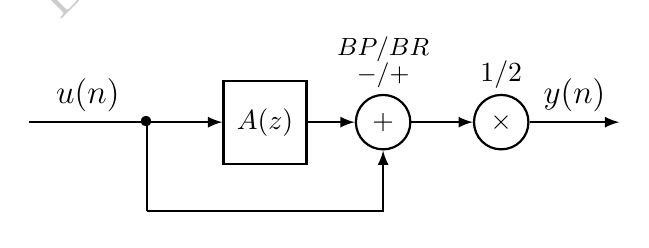
\begin{tikzpicture}[auto, thick, node distance=0.6cm, >=latex, scale = 0.75]
	\draw
	node at (2,0)[delay] (d1) {$A(z)$}
	node at (4,0)[sum] (s1) {$+$} 
	node[above of = s1]{\small$-/+$} node[above of=s1,above=1]{\small{$BP/BR$}}
	node at (6,0) [prod] (p1) {\product} node[above of = p1]{$1/2$};
	
	\draw[-](-2,0) -- node {\large$u(n)$}(0,0);
	\draw[->](0,0) -- node {} (d1);
	\draw[->](d1) -- node {} (s1);
	\draw[->](s1) -- node {} (p1);
	\draw[->](p1) -- node {\large$y(n)$} (8,0);
	\draw[-](0,0) -- node {} (0,-1.5);
	\draw[->](0,-1.5) -| node {} (s1);
	
	\draw
	node at (0,0) {\textbullet};
	\end{tikzpicture}
\end{center}

The difference equations of second-order bandpass filter are
\[
x(n) = u(n) - d(1-c)x(n-1) + cx(n-2)
\]
\[
y(n) = \frac{1+c}{2}x(n) - \frac{1+c}{2}x(n-2),
\]
and corresponding state and output equations are
\[
\begin{bmatrix}x(n)\\x(n-1)\end{bmatrix} = \begin{bmatrix}
-d(1-c)&c\\
1&0
\end{bmatrix}
\begin{bmatrix}x(n-1)\\x(n-2)\end{bmatrix} + \begin{bmatrix}1\\0\end{bmatrix}
u(n)\]
\[
y(n) = \begin{bmatrix}\frac{d(c^2-1)}{2}&\frac{c^2-1}{2}\end{bmatrix}
\begin{bmatrix}x(n-1)\\x(n-2)\end{bmatrix} + \frac{1+c}{2}u(n).
\]
A second-order bandpass filter implementation can be obtained by the following {\bfseries Matlab} code.
\begin{lstlisting}
function y = apbandpassunit(audio, para)
% Applies a bandpass filter to the input signal.
% para(1) is the normalized center frequency in (0,1), i.e. 2*fc/fs.
% para(2) is the normalized bandwidth in (0,1) i.e. 2*fb/fs.
c = (tan(pi*para(2)/2)-1) / (tan(pi*para(2)/2)+1);
d = -cos(pi*para(1));
x = [0; 0];
x_1 = 0;
A = [-d*(1-c), c; 1, 0];
B = [1; 0];
C = [d*(c^2-1)/2, (c^2-1)/2];
D = (1+c)/2;
for n=1:length(audio)
	x_1 = A * x + B * audio(n);
	y(n) = C * x + D * audio(n);
	x = x_1;
end
\end{lstlisting}

The difference equations of second-order bandreject filter are
\[
x(n) = u(n) - d(1-c)x(n-1) + cx(n-2)
\]
\[
y(n) = \frac{1-c}{2}x(n) + d(1-c)x(n-1) + \frac{1-c}{2}x(n-2),
\]
and corresponding state and output equations are
\[
\begin{bmatrix}x(n)\\x(n-1)\end{bmatrix} = \begin{bmatrix}
-d(1-c)&c\\
1&0
\end{bmatrix}
\begin{bmatrix}x(n-1)\\x(n-2)\end{bmatrix} + \begin{bmatrix}1\\0\end{bmatrix}
u(n)\]
\[
y(n) = \begin{bmatrix}\frac{d(1-c^2)}{2}&\frac{1-c^2}{2}\end{bmatrix}
\begin{bmatrix}x(n-1)\\x(n-2)\end{bmatrix} + \frac{1-c}{2}u(n).
\]
A second-order bandreject filter implementation can be obtained by the following {\bfseries Matlab} code.
\begin{lstlisting}
function y = apbandrejectunit(audio, para)
% Applies a bandreject filter to the input signal.
% para(1) is the normalized center frequency in (0,1), i.e. 2*fc/fs.
% para(2) is the normalized bandwidth in (0,1) i.e. 2*fb/fs.
c = (tan(pi*para(2)/2)-1) / (tan(pi*para(2)/2)+1);
d = -cos(pi*para(1));
x = [0; 0];
x_1 = 0;
A = [-d*(1-c), c; 1, 0];
B = [1; 0];
C = [d*(1-c^2)/2, (1-c^2)/2];
D = (1-c)/2;
for n=1:length(audio)
	x_1 = A * x + B * audio(n);
	y(n) = C * x + D * audio(n);
	x = x_1;
end
\end{lstlisting}
\end{document}
